%&"../net"
\endofdump
\tikzexternalize[prefix=cache/]{lab06}
\begin{document}
    \title{Overlay Network and VXLAN}
    \maketitle
    \tableofcontents
    \vfill
    An overlay network can be thought of as a computer network on top of another network. 

    VXLAN is often described as an overlay technology because it allows to stretch Layer 2 connections over an intervening Layer 3 network by encapsulating (tunneling) Ethernet frames in a VXLAN packet that includes IP addresses.
    \vfill
    \clearpage
    \section{建立网络}

    先克隆虚拟机\footnote{感谢 VMWare Workstation 的快照技术,如果重新启动虚拟机,网络配置将会让其无法上网,必须返回原点重新配置。},然后分别在 VM1 和 VM2 上分别运行下面的脚本,得到如图 \ref{fig:topo} 所示的拓扑结构,结果如图 \ref{fig:setup} 所示:

    \code[language=bash]{vm1.sh}
    \code[language=bash]{vm2.sh}

    \begin{figure}[H]
        \centering
        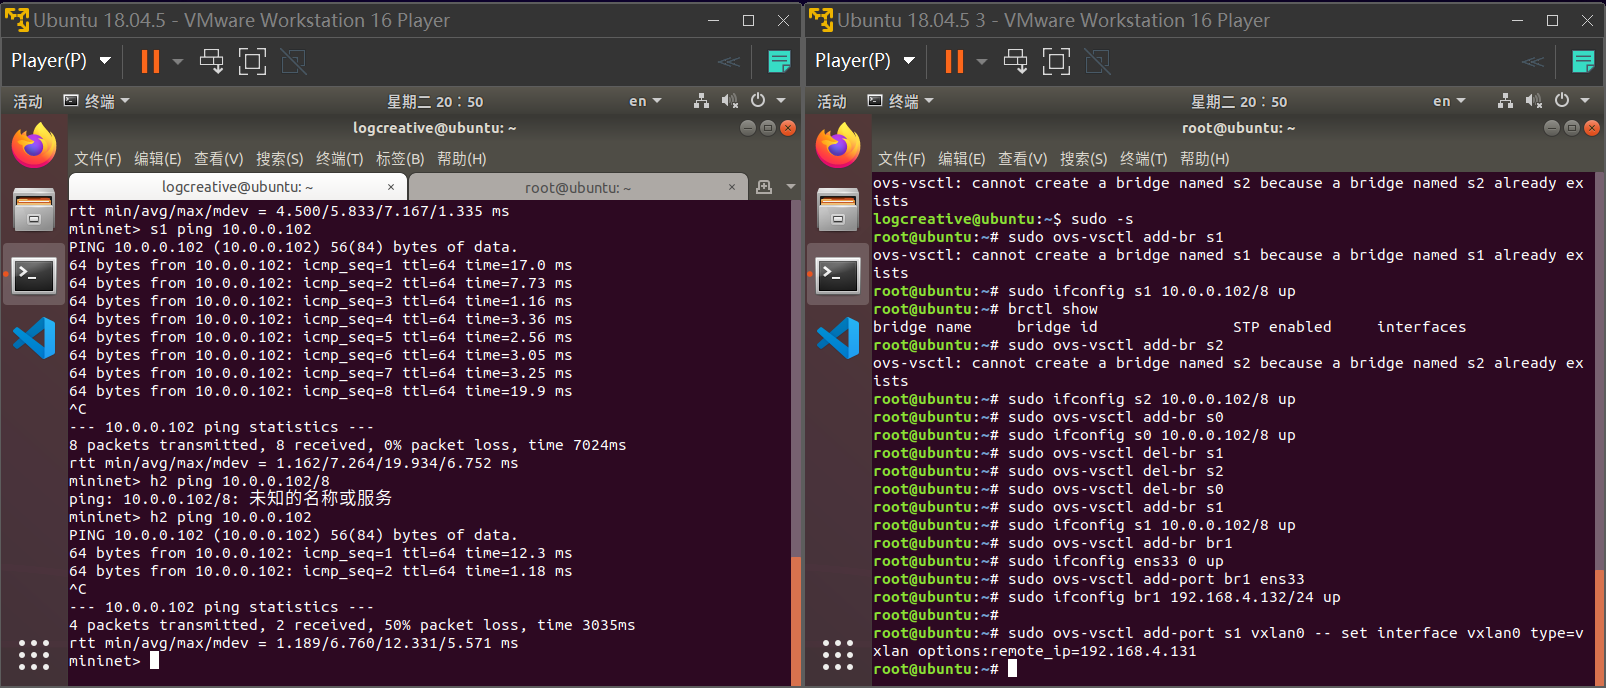
\includegraphics[width=\linewidth]{setup}
        \caption{配置环境}\label{fig:setup}
    \end{figure}

    \begin{figure}[H]
        \centering
        \begin{tikzpicture}
    \tikzstyle{host}=[draw]
    \tikzstyle{switch}=[draw]
    \tikzstyle{connection}=[]
    \tikzstyle{constr}=[right,font=\ttfamily\small]
    
\node (h1) [host] at (-0.5,0.5) {h1};
\node (s1) [switch] at (1.5,0.5) {s1};
\node (s3) [switch] at (3,2) {s3};
\node (s2) [switch] at (4.5,0.5) {s2};
\node (s4) [switch] at (3,-1) {s4};
\node (h2) [host] at (6.5,0.5) {h2};
\draw  (h1) edge (s1);
\draw  (s1) edge (s3);
\draw  (s3) edge (s2);
\draw  (s2) edge (s4);
\draw  (s4) edge (s1);
\draw  (s2) edge (h2);
\end{tikzpicture}
        \caption{拓扑结构}\label{fig:topo}
    \end{figure}

    \section{Wireshark 抓包}
    Use Wireshark to monitor the interfaces s1 and eth0, and describe your findings.

    使用 Wireshark 抓取传输时数据,得到如图 \ref{fig:wireshark} 所示的包。外层为 UDP 报文,显示的实际的 IP 地址;中间为 VXLAN 层;再内侧为 Overlay 的 ICMP 报文,显示的是 Overlay IP 地址。

    \begin{figure}[H]
        \centering
        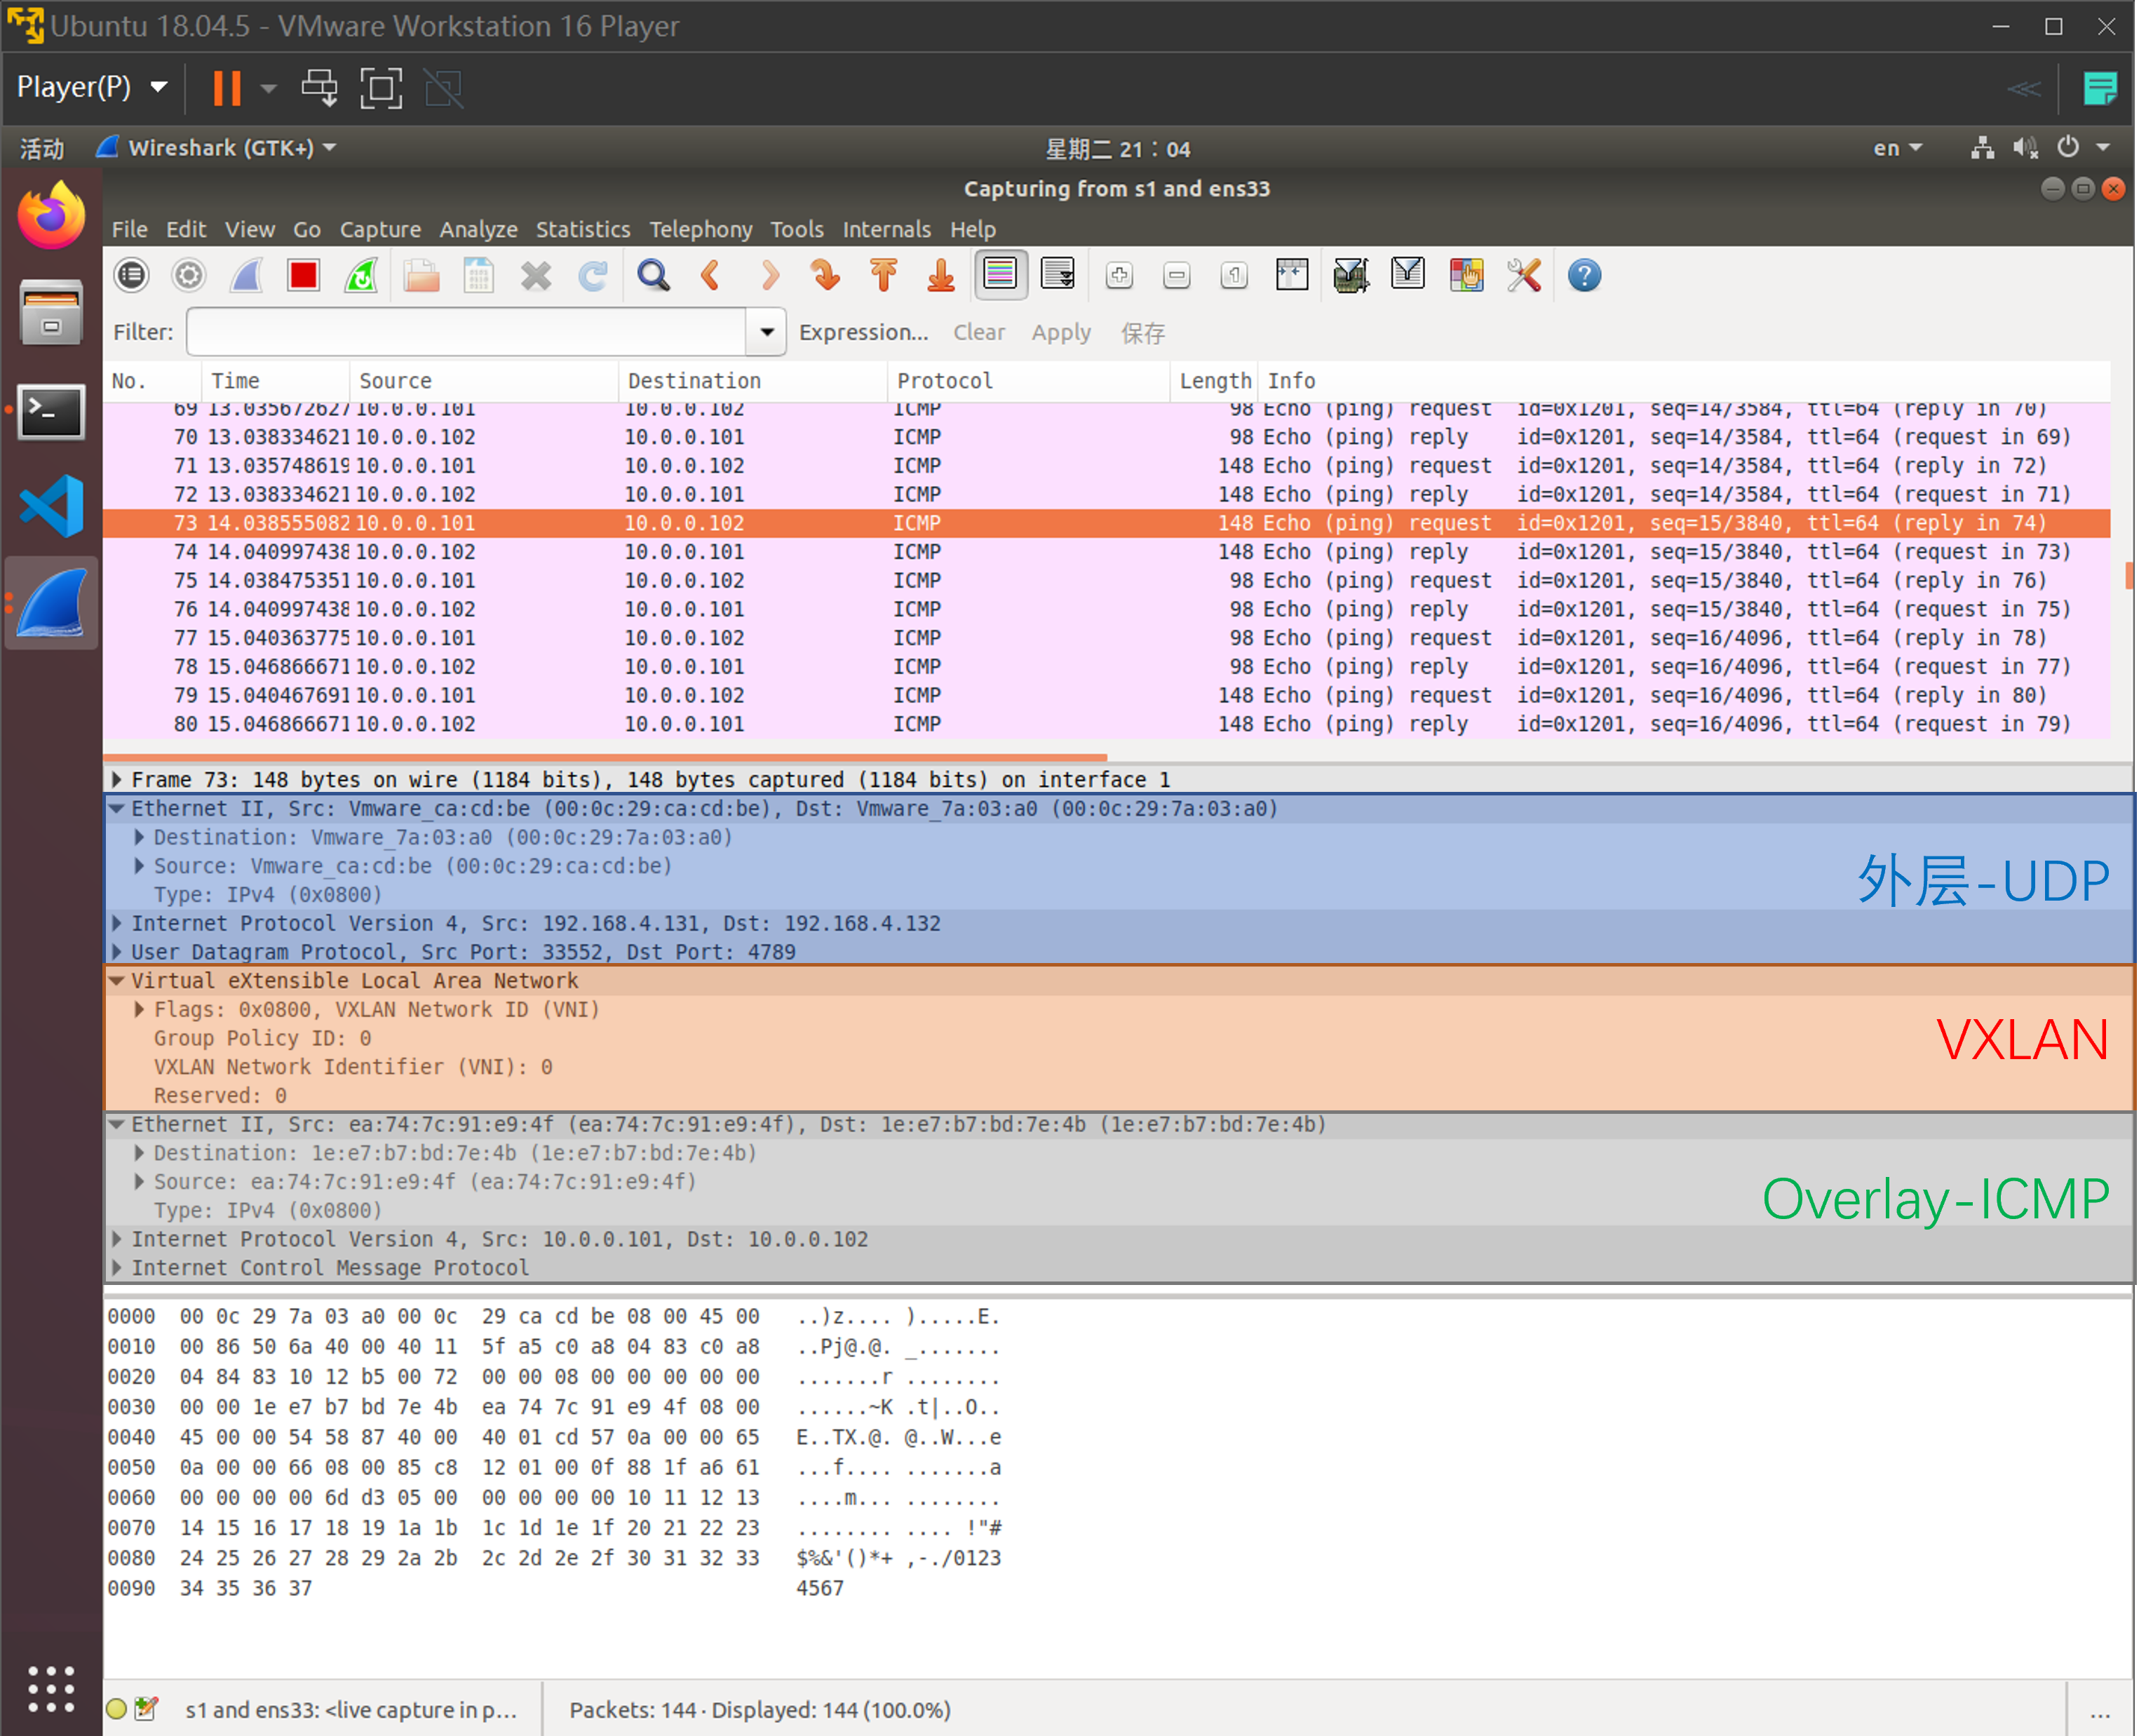
\includegraphics[width=\linewidth]{wireshark}
        \caption{Wireshark 抓包}\label{fig:wireshark}
    \end{figure}

    \section{iperf 测试}
    Use iperf to test the network bandwidth between the two virtual machines 
    \begin{itemize}
        \item Test the bandwidth between 192.168.56.127 and 192.168.56.128
        \item Test the bandwidth between 10.0.0.1/10.0.0.2/10.0.0.101 and 10.0.0.102 (hint: you may need to specify a reasonable MTU size in order for your iperf to work in this case. Please also think about why.)
    \end{itemize}

    Compare the above results and explain the reason. 

    如果不调整 MTU 会导致从 h1 ping 出去的时候只有两个包被接收了,之后会提示“没有可用的缓冲区空间”,如图 \ref{fig:nobuffer} 所示。这是因为 VXLAN 会添加 50 -- 54 Bytes 的额外头部,导致超出 MTU 限制。

    \begin{figure}[H]
        \centering
        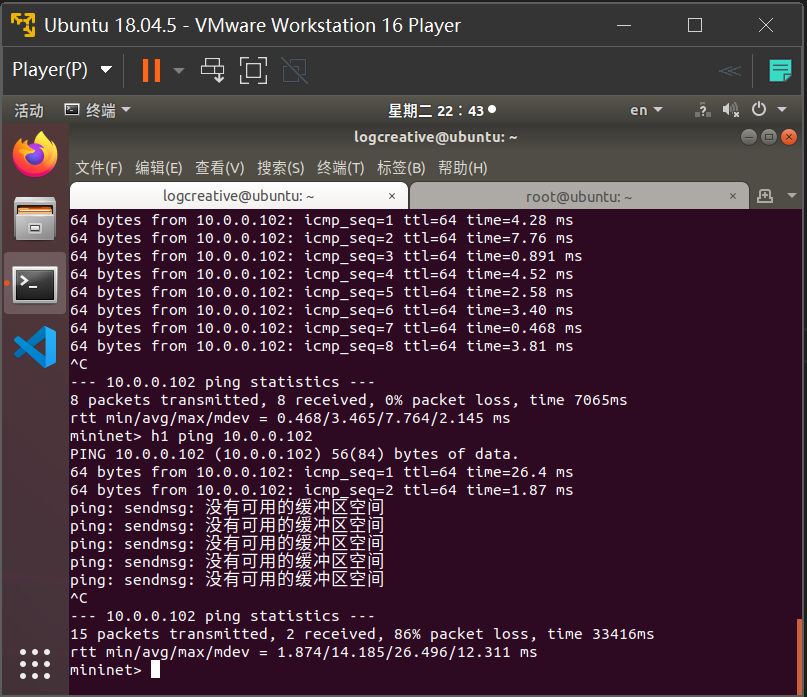
\includegraphics[width=0.7\linewidth]{nobuffer}
        \caption{没有可用的缓冲区空间}\label{fig:nobuffer}
    \end{figure}

    \section{ping 测试}
    Similar to Q2, use ping to test the network latency and analyze your results.
    
\end{document}